\section{Results}
In Table \autoref{tab:table1} we report our results for various classification benchmarks using our implemented BayesBiNN and STE optimizer. We notice that we get a difference of less than 0.1\% as compared to that in the original paper. We generated the results for baseline STE optimizer and full-precision networks by evaluating our implementation of these methods. We also generated the results of PMF, by modifying its original open-sourced code and using the hyperparameters mentioned in the original paper.

\begin{figure}[h]
     \centering
     \begin{subfigure}[b]{0.3\textwidth}
         \centering
         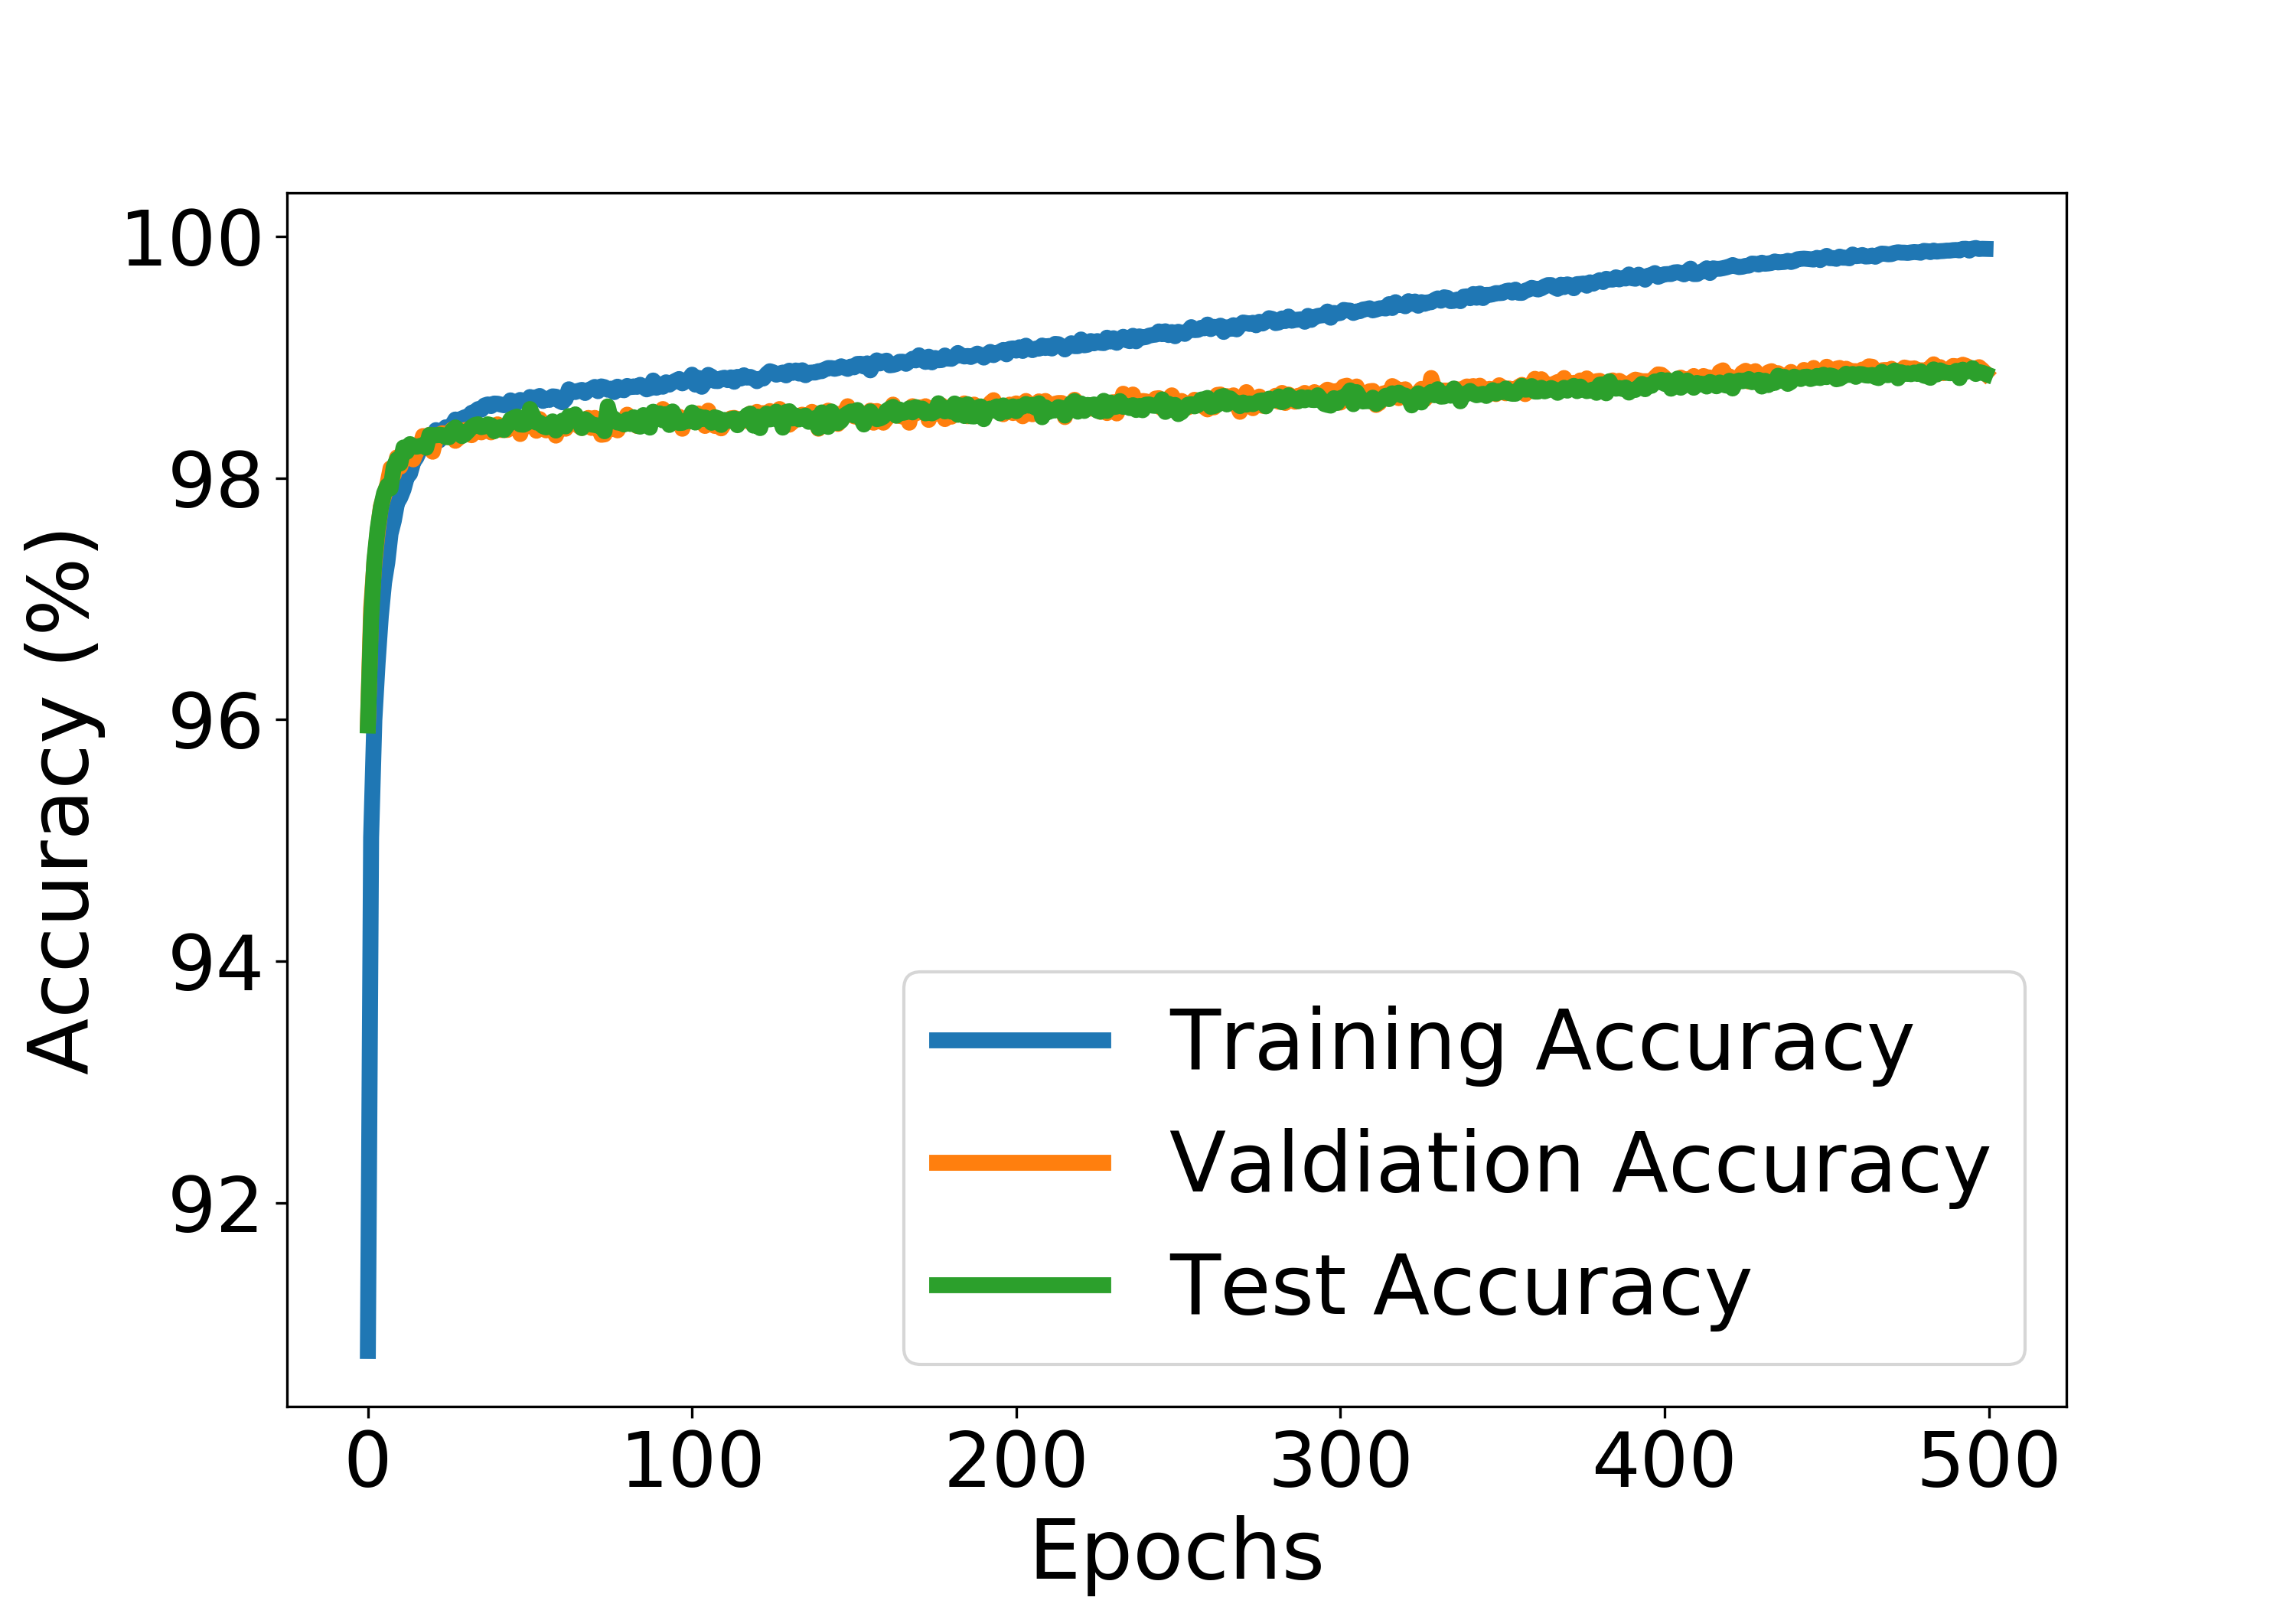
\includegraphics[width=1.2\textwidth]{../openreview/figs/MNIST.png}
         \caption{MNIST}
     \end{subfigure}
     \hfill
     \begin{subfigure}[b]{0.3\textwidth}
         \centering
         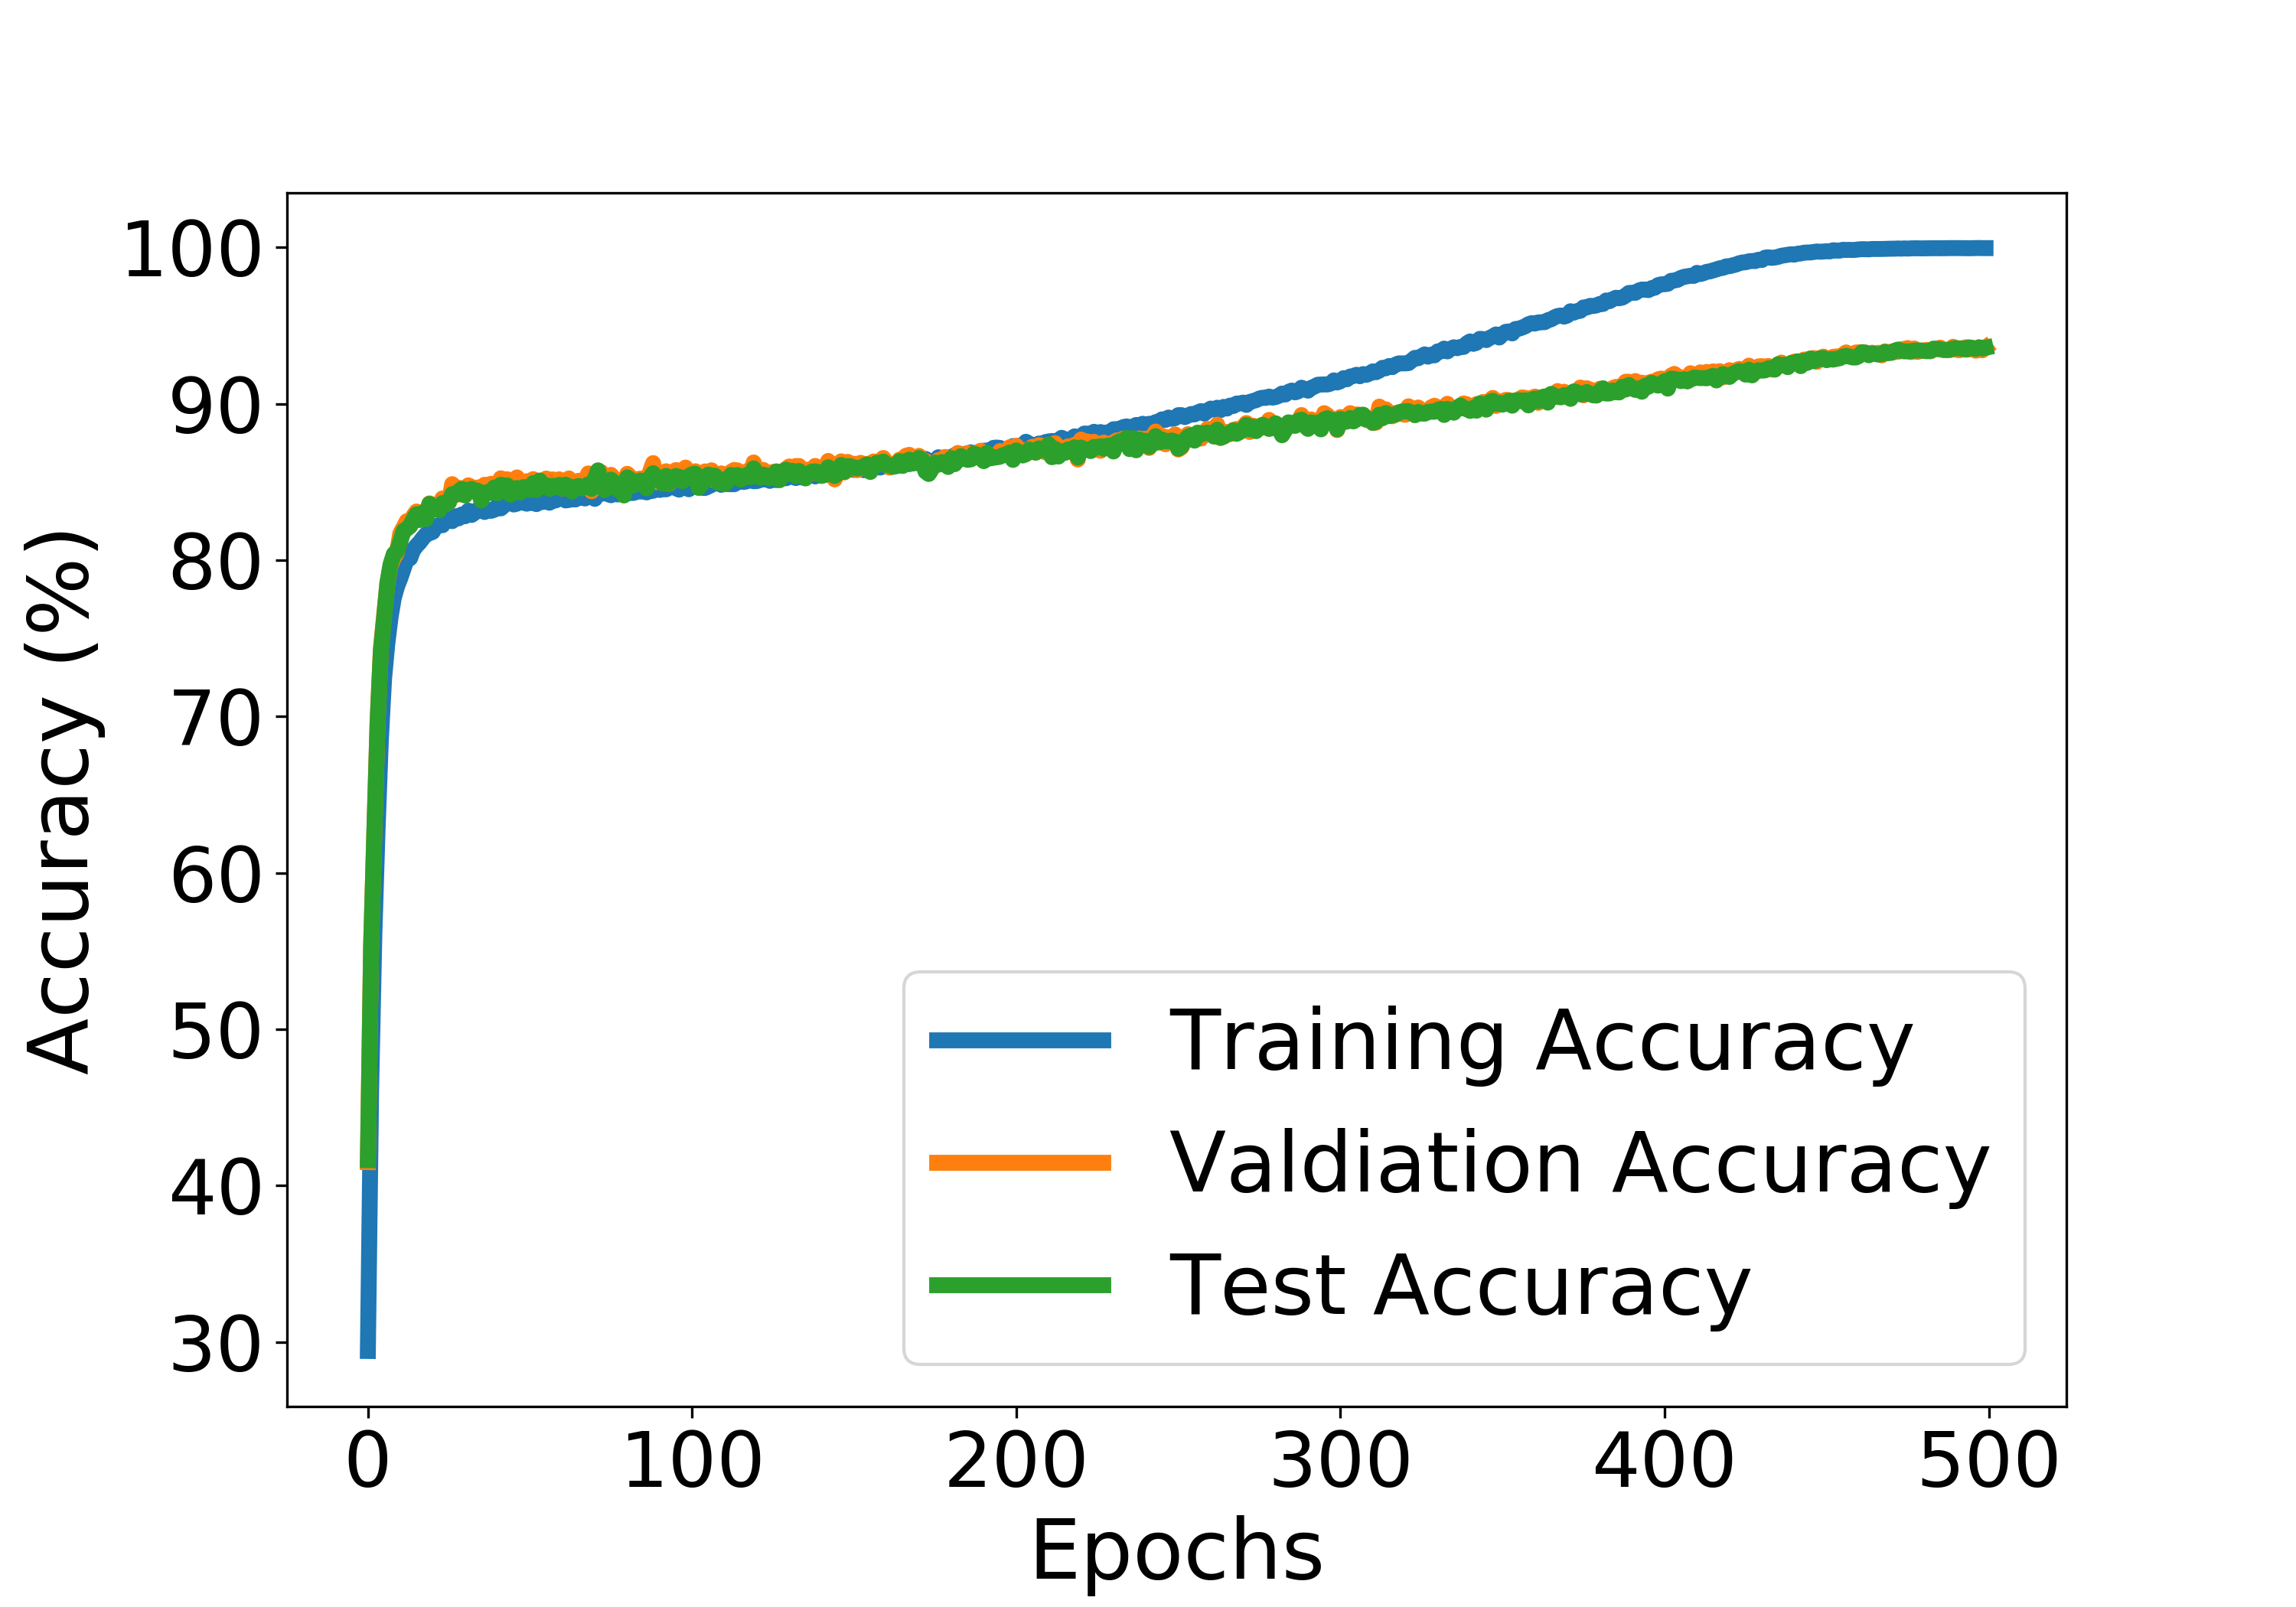
\includegraphics[width=1.2\textwidth]{../openreview/figs/CIFAR10.png}
         \caption{CIFAR10}
     \end{subfigure}
     \hfill
     \begin{subfigure}[b]{0.3\textwidth}
         \centering
         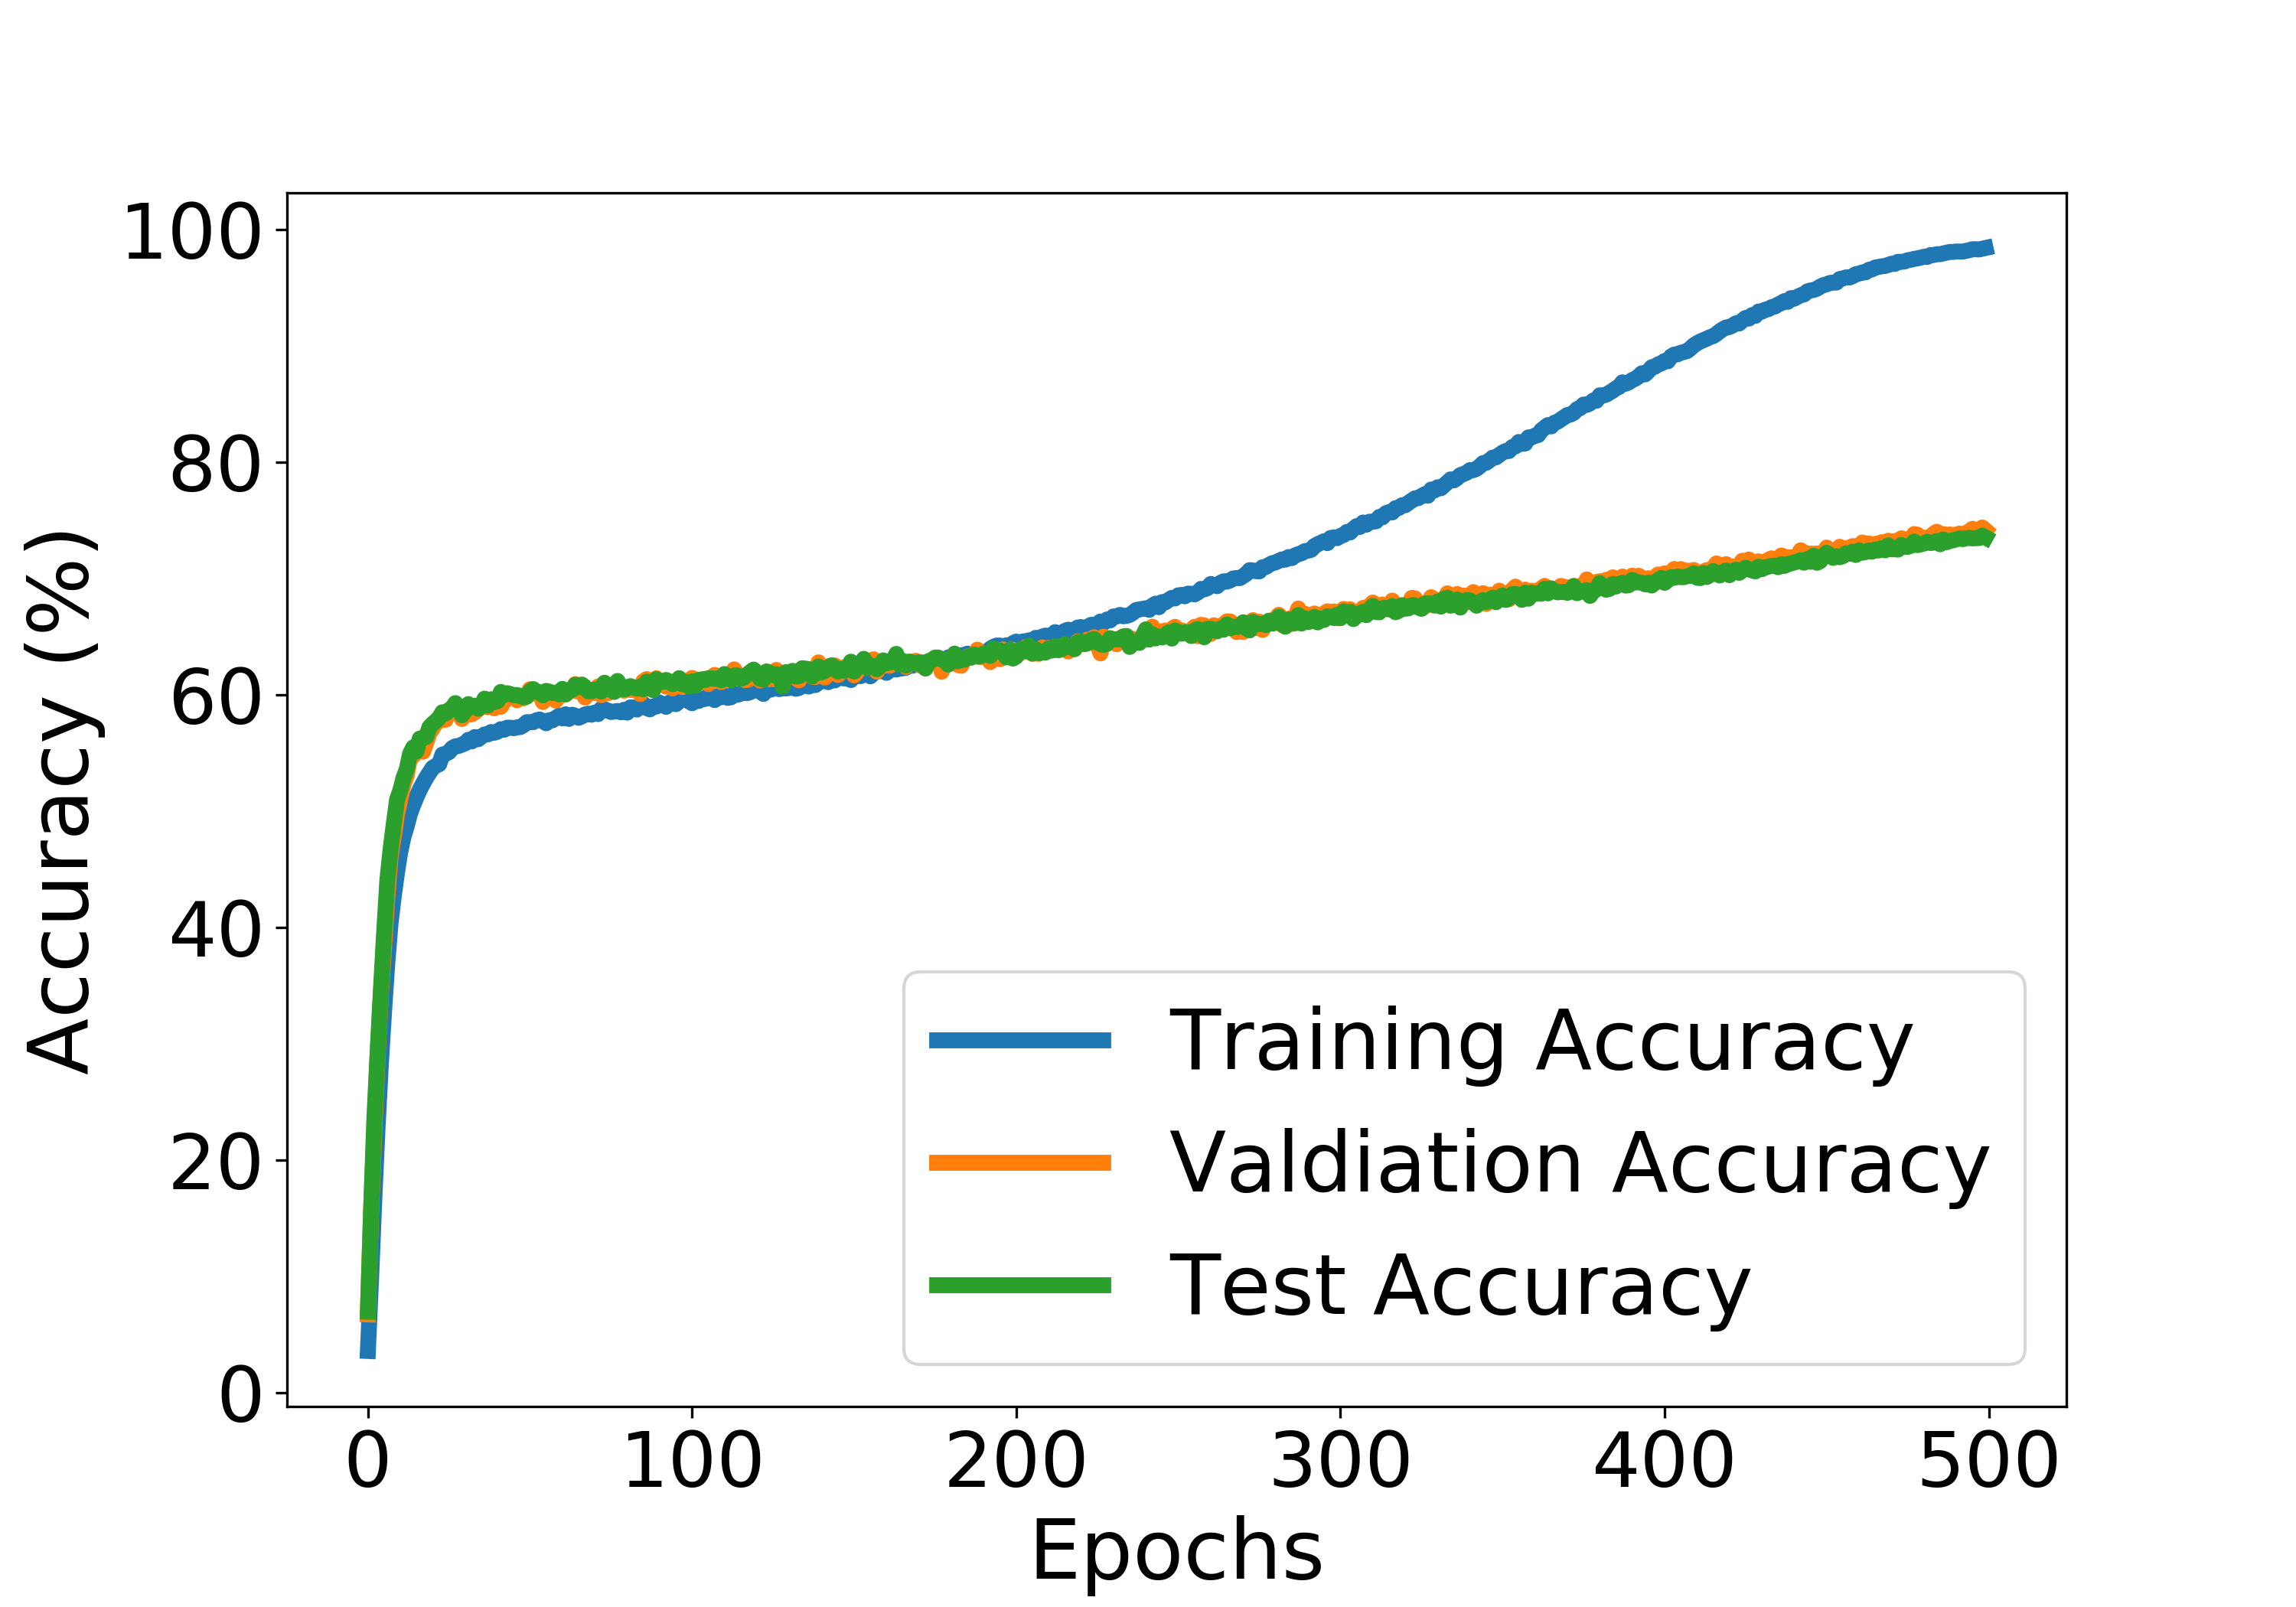
\includegraphics[width=1.2\textwidth]{../openreview/figs/CIFAR100.png}
         \caption{CIFAR100}
     \end{subfigure}
        \caption{Training/Validation/Test accuracy using BayesBiNN optimizer}
\end{figure}

\begin{table}[h]
\begin{center}
\small
\begin{tabular}{ | c | c | c | c | c | }
\hline
 Datasets & Optimizer & Training Accuracy & Validation Accuracy & Test Accuracy \\ \hline
  \multirow{5}{4em}{MNIST} 
   & BayesBiNN(ours) & $99.90 \pm 0.01\%$ & $99.89 \pm 0.07\%$ & $98.87 \pm 0.06\%$  \\
   & BayesBiNN(orig.) & $99.85 \pm 0.05\%$ & $99.02 \pm 0.13\%$ & $98.86 \pm 0.05\%$  \\
   & STE & $99.90 \pm 0.01\%$ & $98.86 \pm 0.09\%$ & $98.89 \pm 0.05\%$  \\
   & PMF & - & $98.73\%$ & -  \\
   & Adam (Full Precision) & $99.98 \pm 0.01\%$ & $99.02 \pm 0.04\%$ & $99.02 \pm 0.01\%$  \\ 
\hline

  \multirow{5}{4em}{CIFAR10}
   & BayesBiNN(ours) & $99.96 \pm 0.01\%$ & $93.59 \pm 0.45\%$ & $93.54 \pm 0.26\%$  \\
   & BayesBiNN(orig.) & $99.96 \pm 0.01\%$ & $94.23 \pm 0.41\%$ & $93.72 \pm 0.16\%$  \\
   & STE & $99.99 \pm 0.01\%$ & $93.77 \pm 0.06\%$ & $93.54 \pm 0.08\%$  \\
   & PMF & - & $91.98\%$ & -  \\
   & Adam (Full Precision) & $99.99 \pm 0.01\%$ & $94.27 \pm 0.15\%$ & $94.38 \pm 0.16\%$  \\ 
\hline
   
   
  \multirow{5}{4em}{CIFAR100} 
   & BayesBiNN(ours) & $98.35 \pm 0.1\%$ & $74.13 \pm 0.78\%$ & $73.56 \pm 0.06 \%$ \\
   & BayesBiNN(orig.) & $98.02 \pm 0.18\%$ & $74.76 \pm 0.41\%$ & $73.68 \pm 0.31\%$  \\
   & STE & $99.22 \pm 0.03\%$ & $72.74 \pm 0.06\%$ & $73.25 \pm 0.26\%$  \\
   & PMF & - & $70.82\%$ & -  \\
   & Adam (Full Precision) & $99.89 \pm 0.02\%$ & $75.04 \pm 0.71\%$ & $74.80 \pm 0.39\%$  \\ \hline
\end{tabular}
\caption{Results of different optimizers trained on MNIST, CIFAR10, and CIFAR100.}
\label{tab:result_1}

\end{center}
\end{table}

\subsection{Comparison with LR-Net}
Authors compared their BayesBiNN approach to the LR-Net method presented in \citet{r8}. We tried to reproduce the result for the same setting. In this comparison, the data pre-processing and augmentation methods remain the same as mentioned in section 4.2, but we do not split the data in training and validation sets in this case. We denote the test accuracies after 190 epochs in the case of MNIST and 290 epochs in the case of CIFAR-10, as done in the original paper to maintain uniformity. Note that, our accuracy is matching with that of the original authors in the case of MNIST but not in the case of CIFAR-10. We suspect that this is due to some difference in Batch-Norm layers used.

\begin{table}[h]
\begin{center}
\renewcommand{\arraystretch}{1.1}
\begin{tabular}{ | c | c | c |}
\hline
 Optimizer & MNIST &  CIFAR10 \\ \hline
%   \multirow{2}{5em}{MNIST} 
   BayesBiNN (ours) & \textbf{99.52\%} & $84.49\%$ \\ \hline
   BayesBiNN (orig.) & $99.50\%$ & $\textbf{93.97\%}$ \\ \hline
   LR-net \citet{r8} & $99.47\%$ & $93.18\%$ \\
\hline
\end{tabular}
\caption{Test accuracy of BayesBiNN and LRNet.}
\label{tab:LR_result_2}

\end{center}
\end{table}

\subsection{Continual Learning}
As mentioned in the original paper, we try to reproduce the author's claims about weight distribution across tasks in a simple continual learning domain tested on Permuted MNIST. Clearly, as we learn across the tasks, the curve becomes flat from the middle conveying that the weights become more deterministic. Our result matches with the claims in the original paper.
\begin{figure}[h]
     \centering
     \begin{subfigure}[b]{0.3\textwidth}
         \centering
         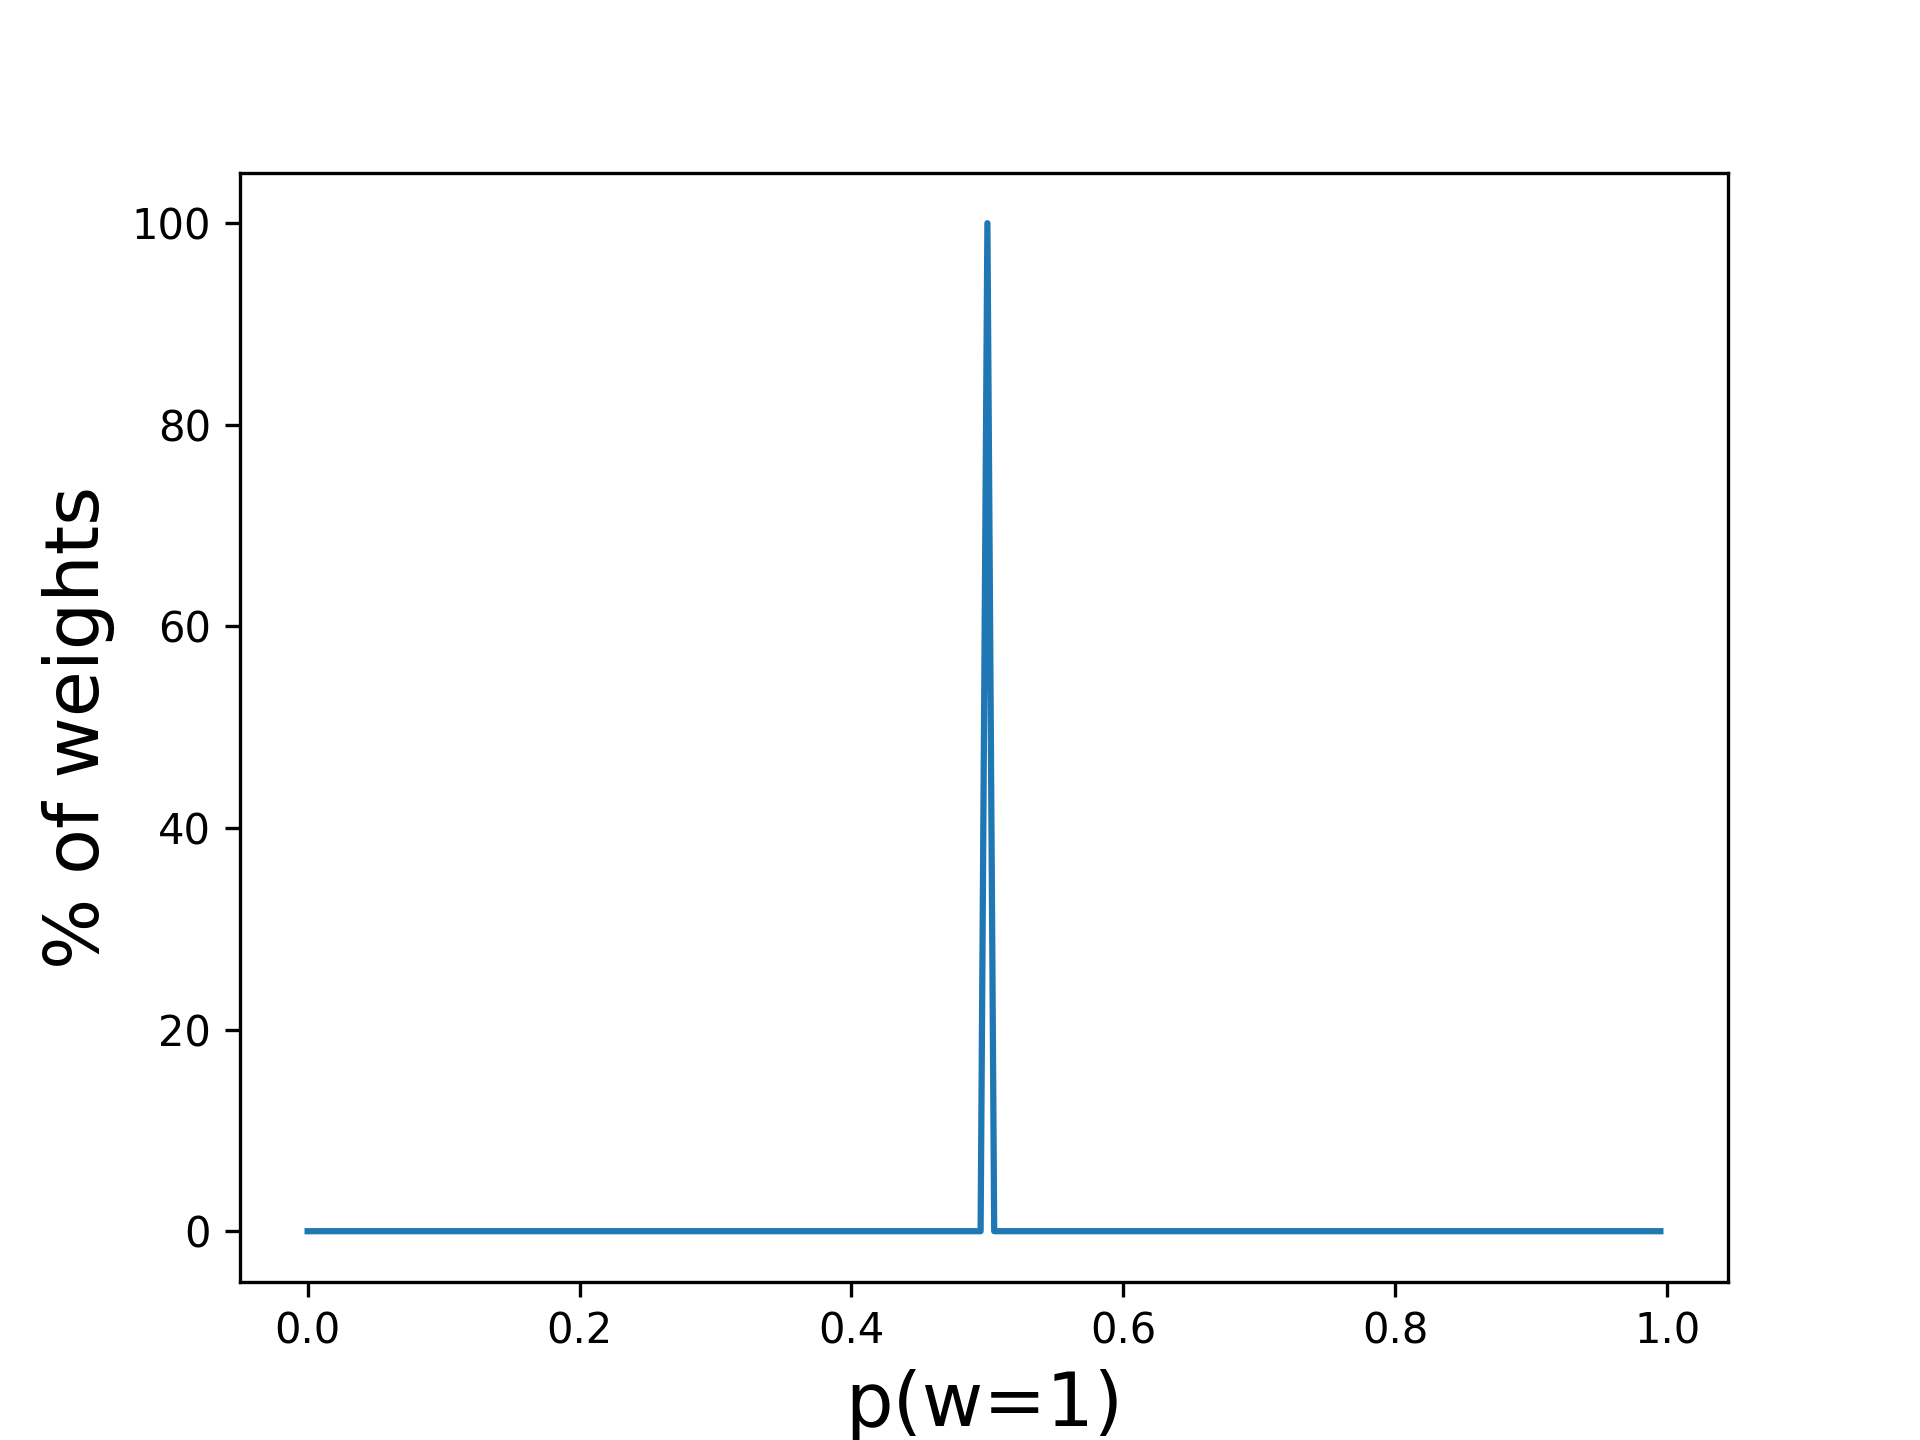
\includegraphics[width=1.1\textwidth]{../openreview/figs/after_task_0.png}
         \caption{Prior $\lambda$}
     \end{subfigure}
     \hfill
     \begin{subfigure}[b]{0.3\textwidth}
         \centering
         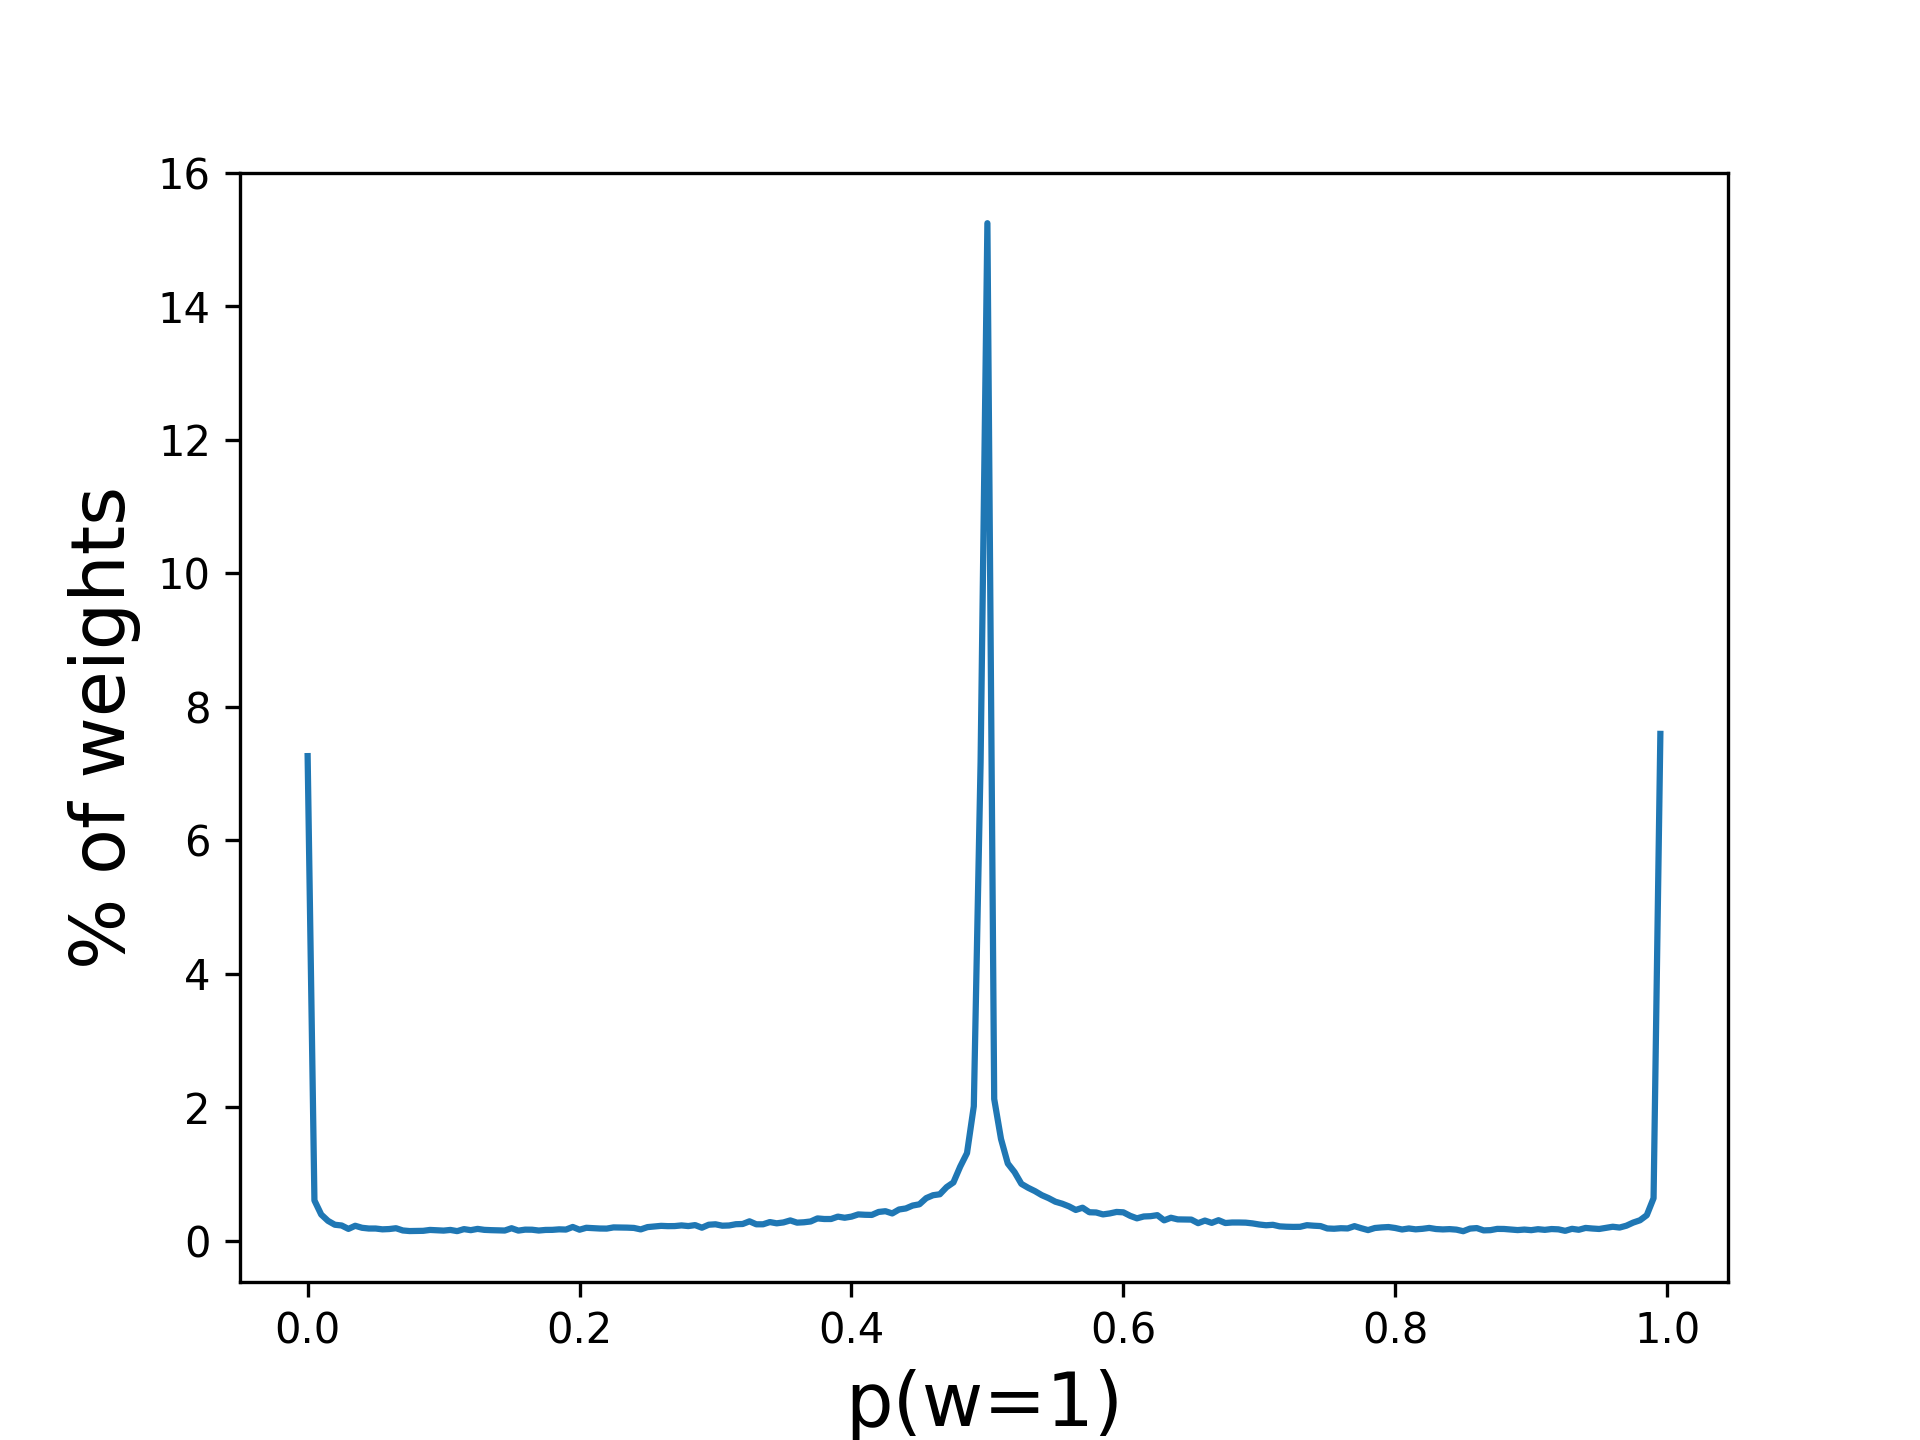
\includegraphics[width=1.1\textwidth]{../openreview/figs/after_task_1.png}
         \caption{$\lambda$ after task 1}
     \end{subfigure}
     \hfill
     \begin{subfigure}[b]{0.3\textwidth}
         \centering
         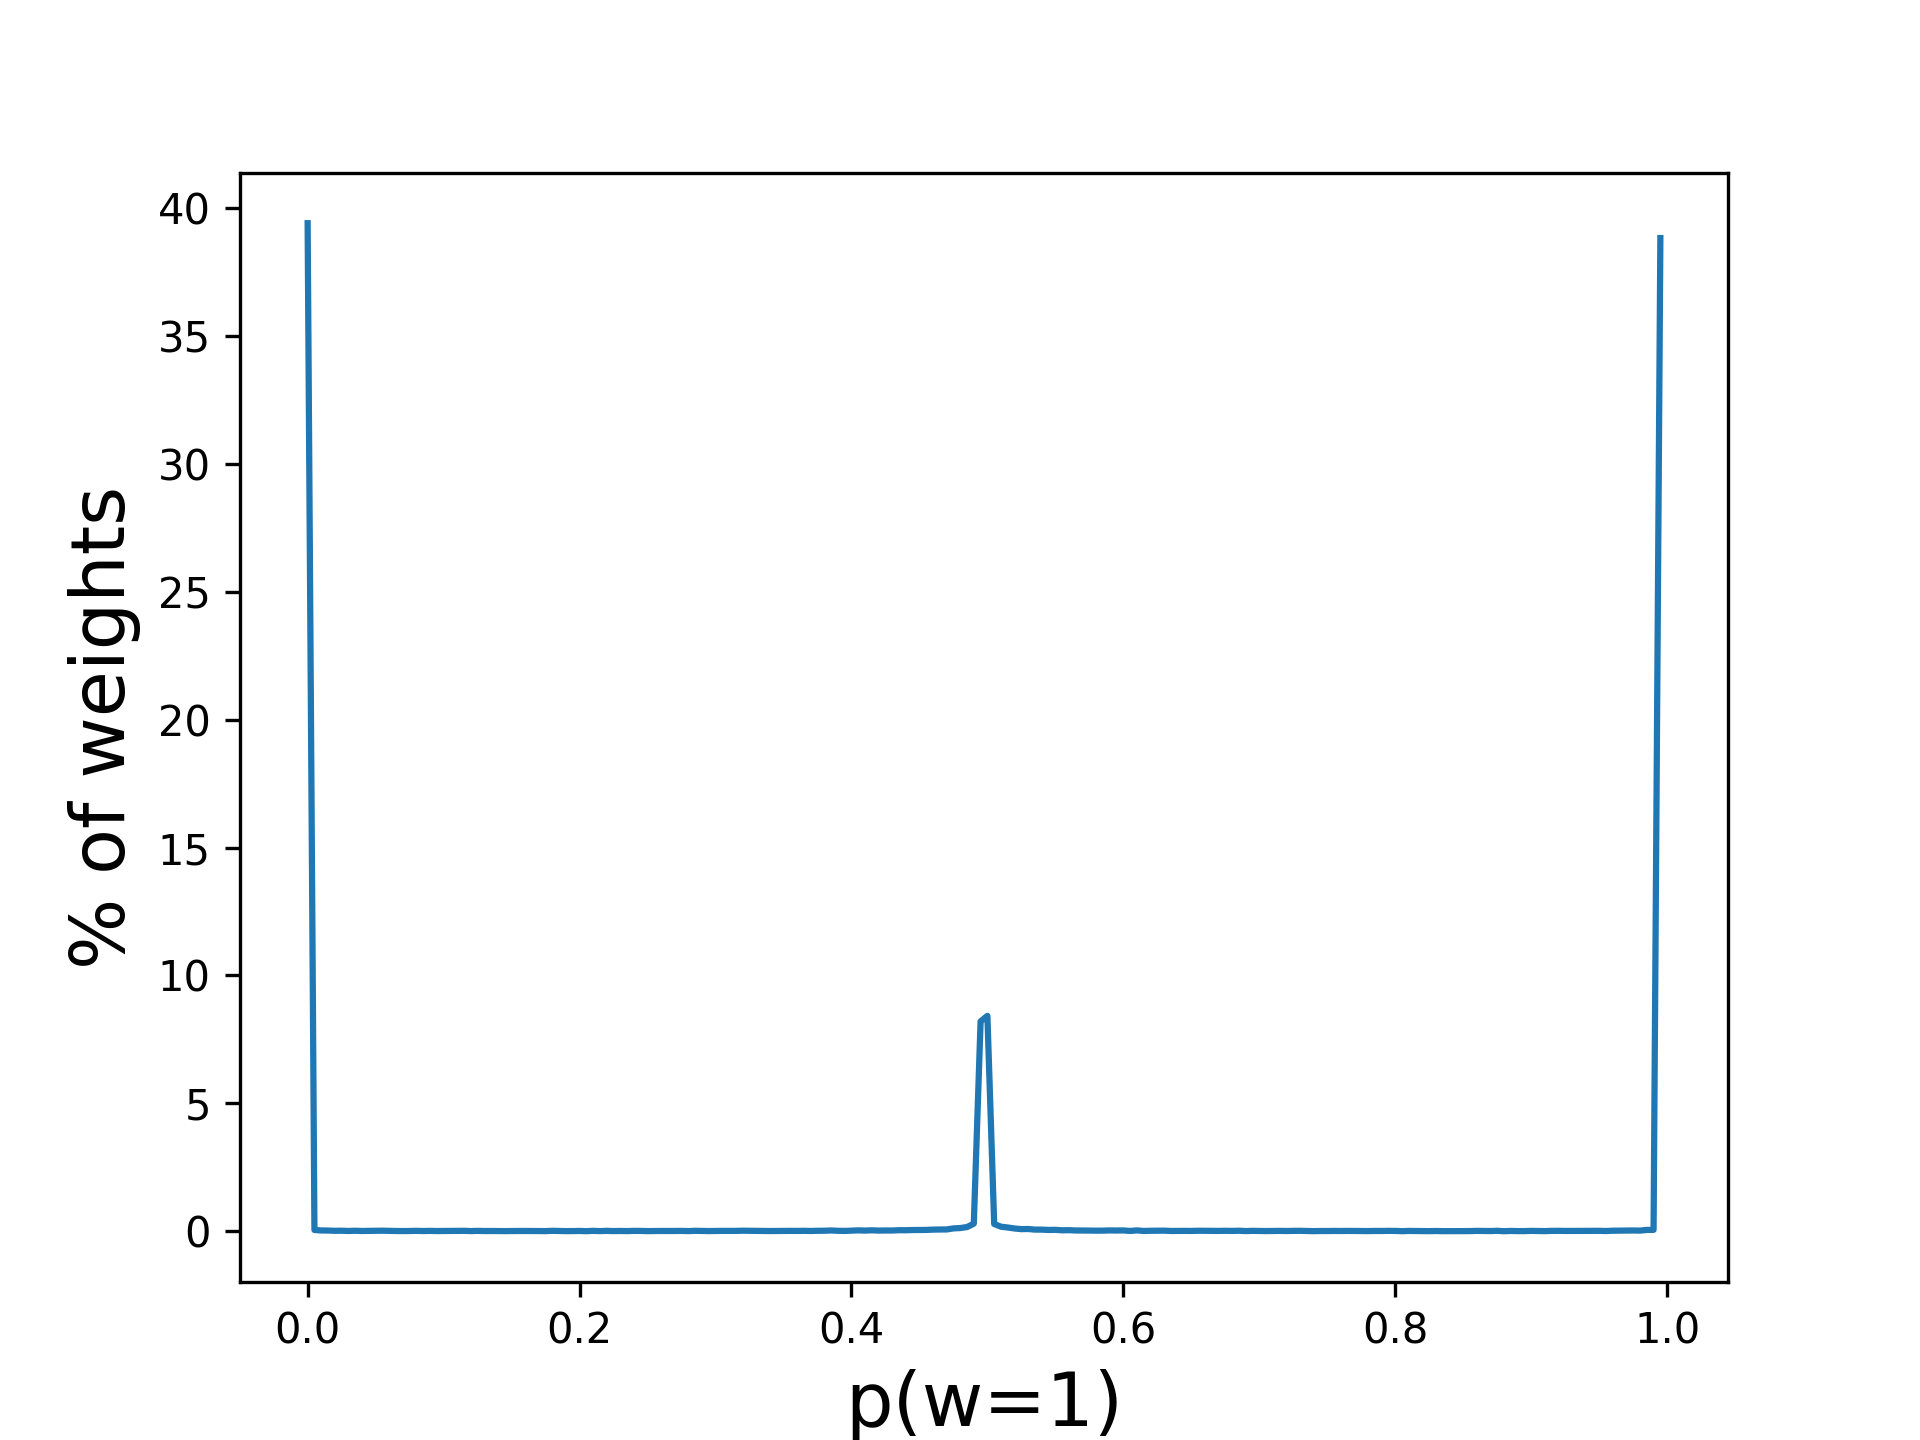
\includegraphics[width=1.1\textwidth]{../openreview/figs/after_task_2.png}
         \caption{$\lambda$ after task 2}
     \end{subfigure}
        \caption{Distribution of $p(w=1)$ across consecutive learning tasks}
\end{figure}

\subsection{Visualization using Synthetic Dataset}

In the original paper, the authors present visualizations on binary classification (Two moons dataset \citet{r10}) and toy regression (Snelson dataset \citet{r9}) using STE and BayesBiNN optimizer. For the classification task, the authors claimed that STE is a more deterministic classifier compared to BayesBiNN. We reproduced this experiment and the results depicted in Figure \autoref{fig3} seem to be consistent with the author's claim. For the regression task, we conclude that the author's claim about BayesBiNN (mean) giving a smoother curve compared to STE is true, which can also be seen in Figure \autoref{fig4}. 


\begin{figure}[h]
     \centering
         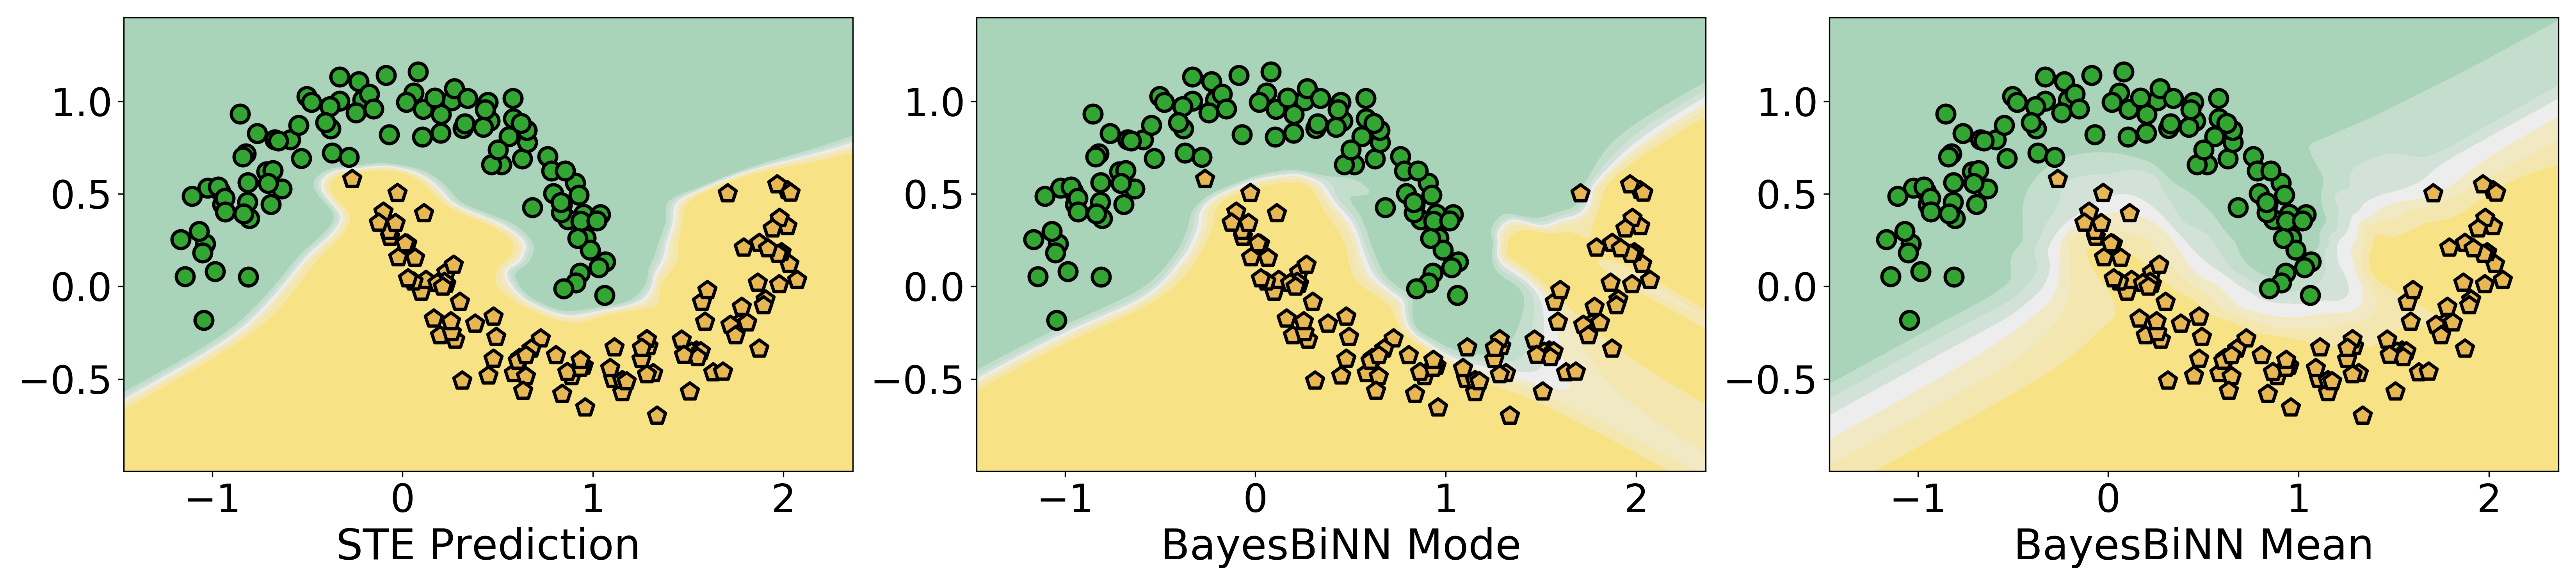
\includegraphics[width=1\textwidth]{../openreview/figs/TwoMoon.png}
         \caption{Classification on Two Moons dataset using STE and BayesBiNN optimizer.}
         \label{fig3}
\end{figure}

\begin{figure}[h]
     \centering
         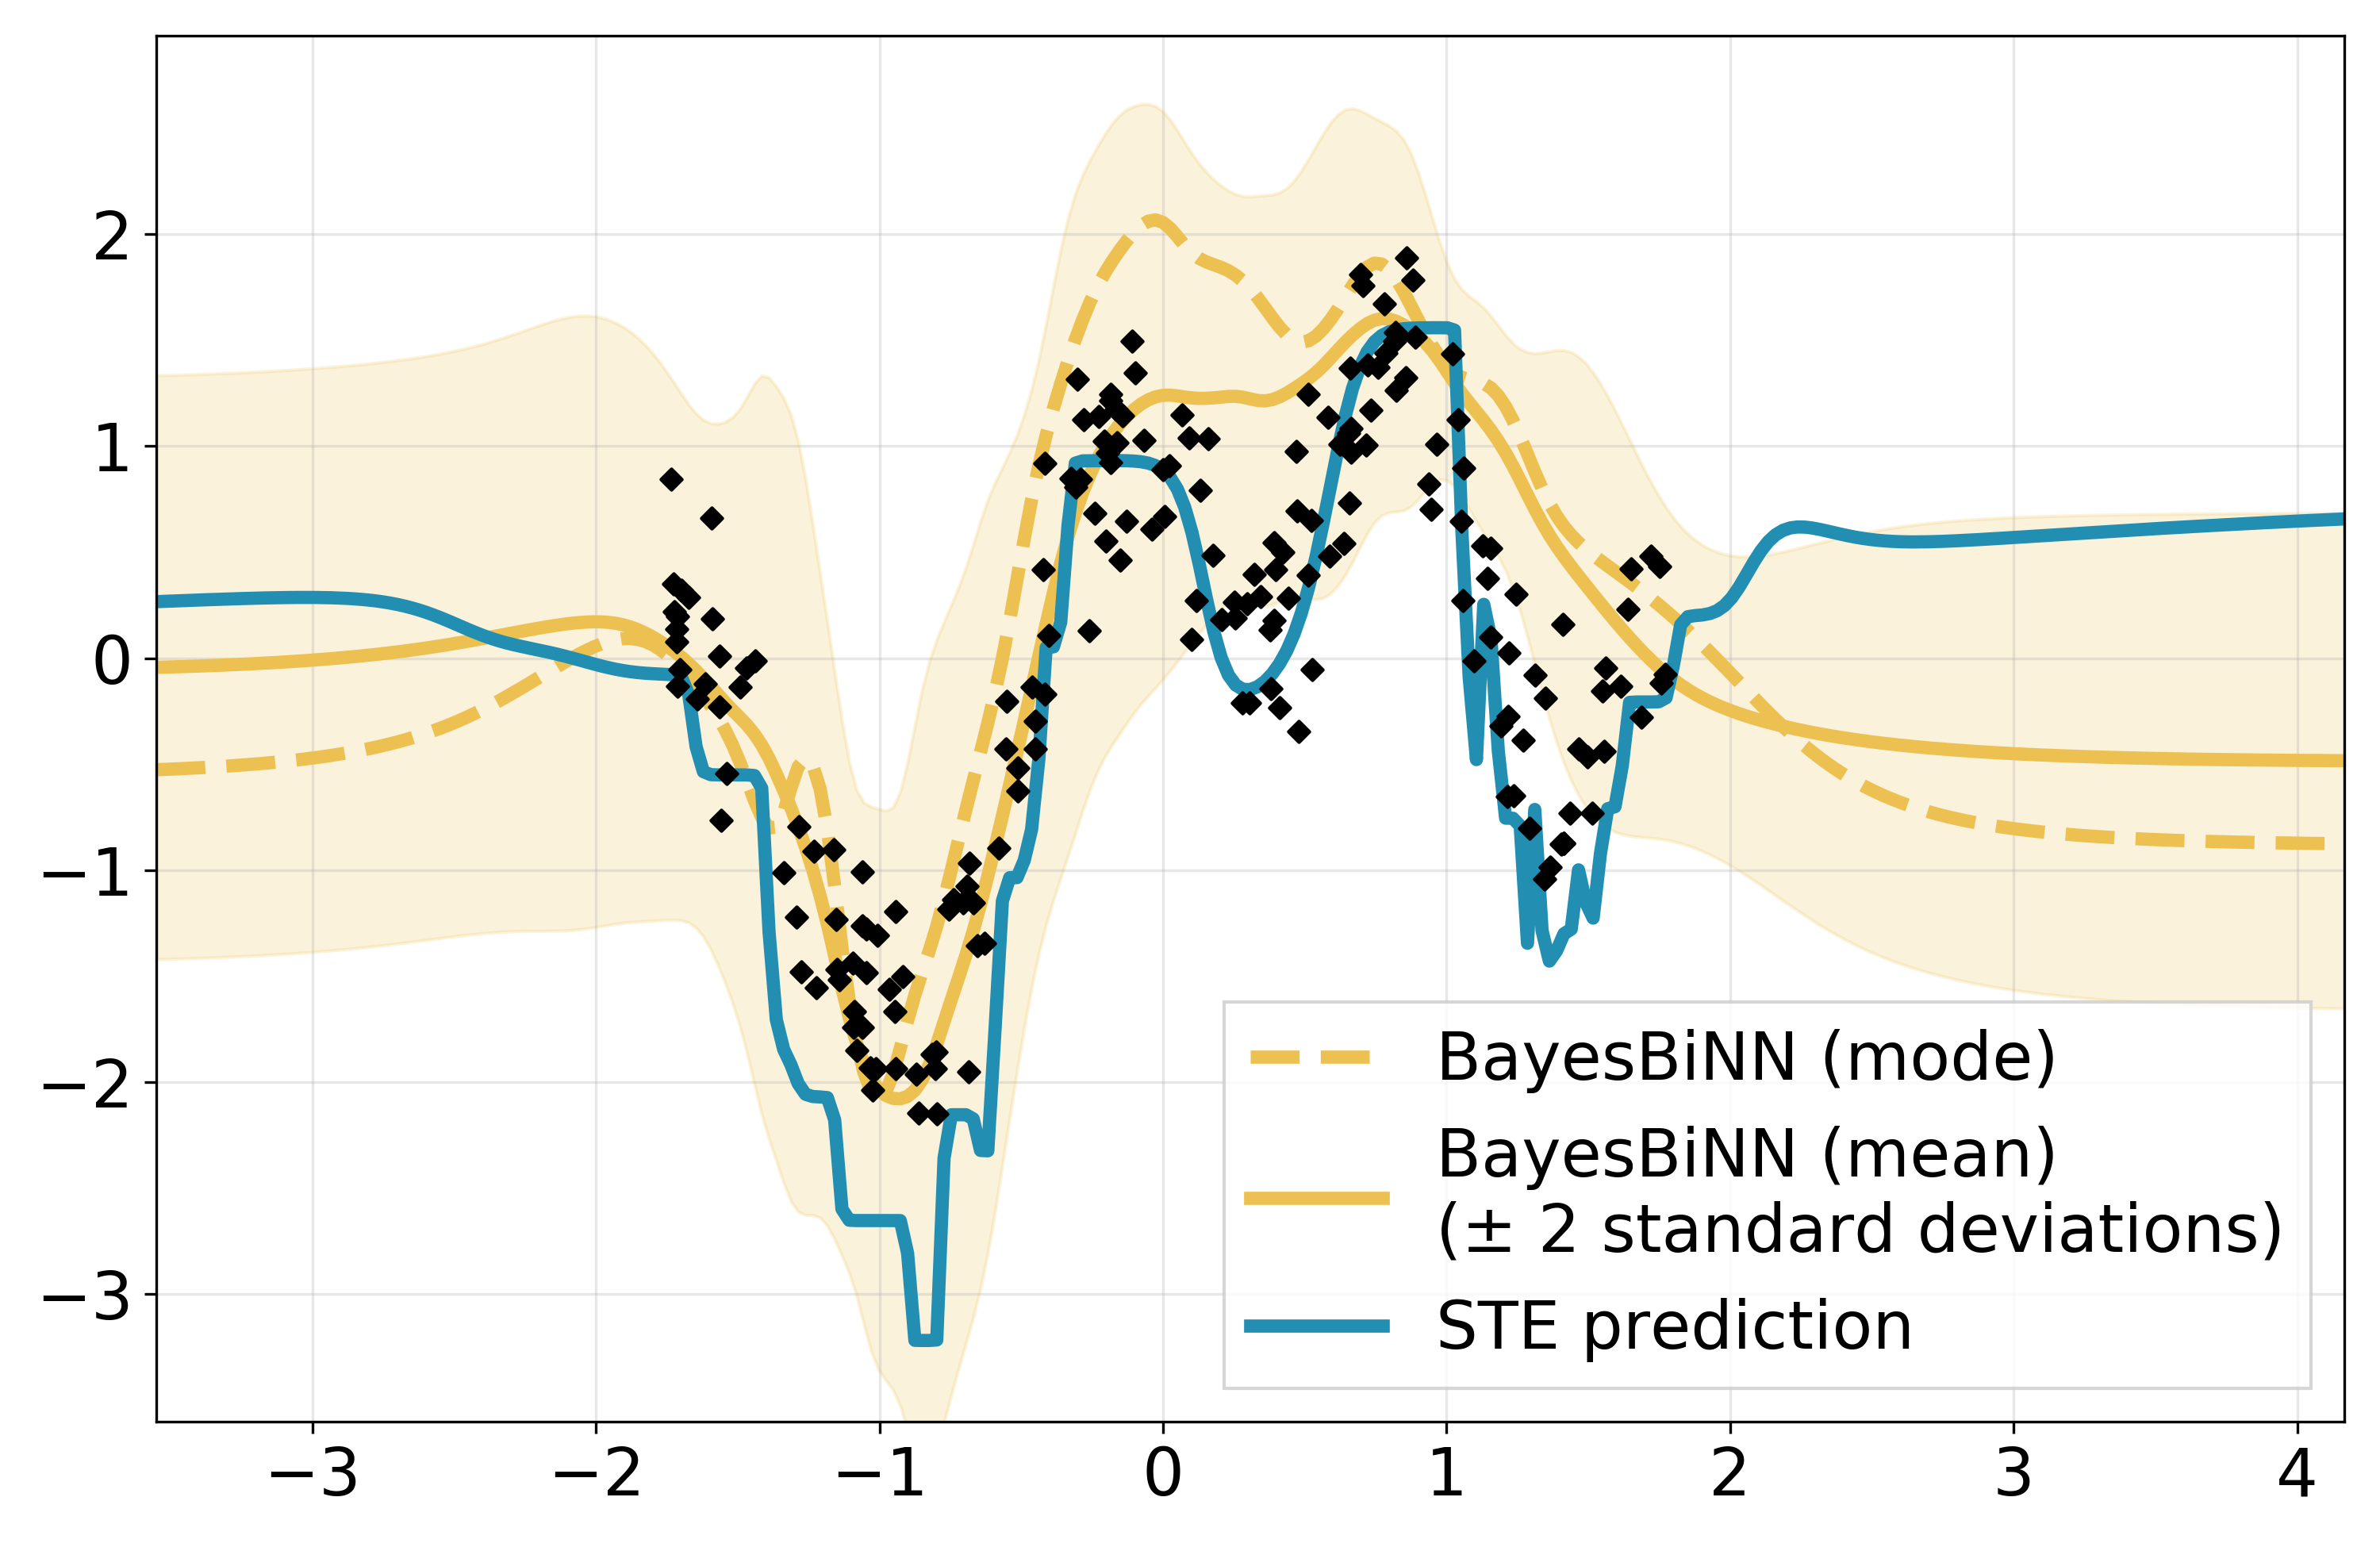
\includegraphics[width=0.6\textwidth]{../openreview/figs/Snelson.png}
         \caption{Regression on Snelson dataset using STE and BayesBiNN optimizer.}
         \label{fig4}
\end{figure}


\begin{table}[h]
\begin{center}
\setlength{\tabcolsep}{12pt}
\renewcommand{\arraystretch}{1.3}
\begin{tabular}{ | c | c | c | c | c | c | c | }
\hline
 \textbf{Temperature} & 10 & 1 & 0.1 & $10^{-2}$ & $10^{-3}$ & $10^{-4}$ \\\hline
 MSE Loss & 1.313 & 0.208 & 2.151 & 0.443 & 0.231 & 0.199\\ \hline
 \textbf{Temperature} & $10^{-5}$ & $10^{-6}$ & $10^{-7}$ & $10^{-8}$ & $10^{-9}$ & $10^{-10}$\\  \hline
 MSE Loss & 0.156 & 0.127 & 0.173 & 0.122 & 0.195 & 0.173\\ 
\hline
\end{tabular}
\caption{Mean square error loss of Snelson dataset for different temperatures.}
\label{tab:Ablation_result_4}

\end{center}
\end{table}

\subsection{Extended Results (Semantic Segmentation)}
We tried to validate the performance of the BayesBiNN optimizer on more complex tasks like semantic segmentation. Unfortunately, the results with BayesBiNN were quite underwhelming as compared to STE and its full-precision counterpart. We tried various parameters to improve its performance but none seemed to work. We had a brief discussion with the authors regarding this issue and the authors suggested that Bayesian models are intrinsically very difficult to train. For the results shown in Table \autoref{tab:table5} and Figure \autoref{fig5}, we have used the hyperparameters denoted in Table \autoref{tab:table1}.

\begin{table}[h]
\begin{center}
\renewcommand{\arraystretch}{1.1}
\begin{tabular}{ | c | c | c | c |}
\hline
  & BayesBiNN & STE &  Adam (Full Precision) \\ \hline
    Validation Score & 0.4102 & 0.3108 & 0.2943 \\ \hline
\end{tabular}
\caption{(1 - IoU) score for validation set}
\label{tab:table5}
\end{center}
\end{table}

\begin{figure}[h]
     \centering
     \begin{subfigure}[b]{0.3\textwidth}
         \centering
         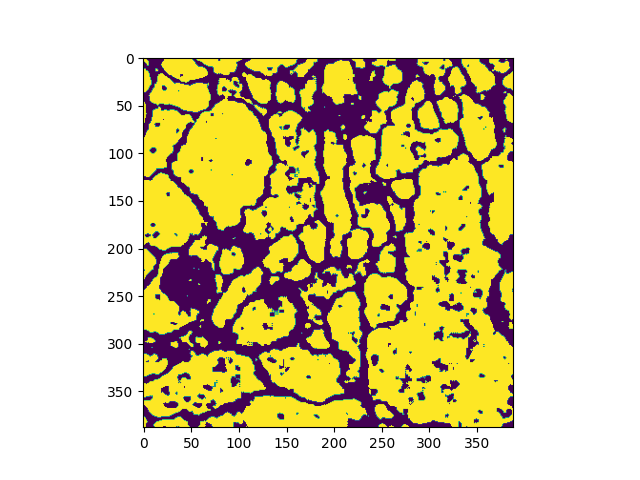
\includegraphics[width=1.3\textwidth]{../openreview/figs/output_bayesbinn.png}
         \caption{BayesBiNN}
     \end{subfigure}
     \hfill
     \begin{subfigure}[b]{0.3\textwidth}
         \centering
         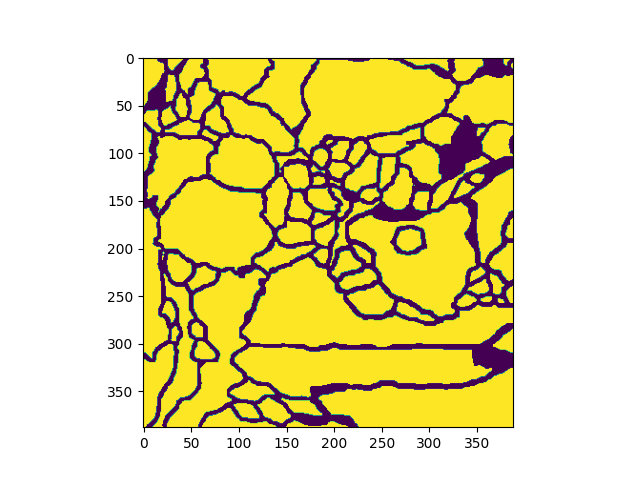
\includegraphics[width=1.3\textwidth]{../openreview/figs/output_ste.png}
         \caption{STE}
     \end{subfigure}
     \hfill
     \begin{subfigure}[b]{0.3\textwidth}
         \centering
         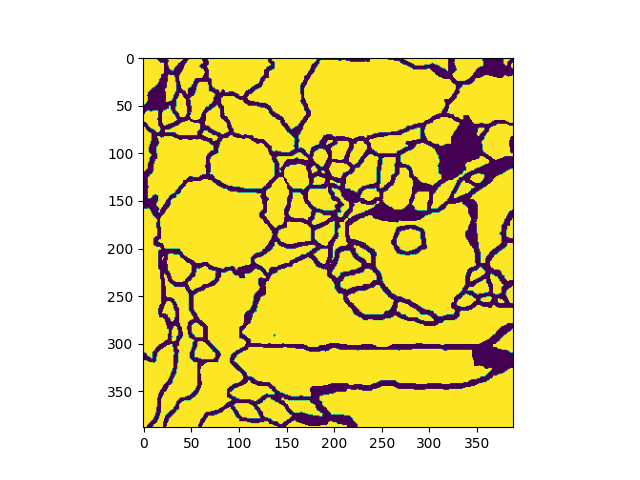
\includegraphics[width=1.3\textwidth]{../openreview/figs/output_normal.png}
         \caption{Adam}
     \end{subfigure}
        \caption{Some samples of segmented image outputs}
        \label{fig5}
\end{figure}